%*----------- SLIDE -------------------------------------------------------------
\begin{frame}[t]{Melhoria na busca de artigos}
    \framesubtitle{Existe algum método eficiente?}
    %\transboxin[duration=1,direction=30]
    A biblioteconomia.

    \begin{figure}
        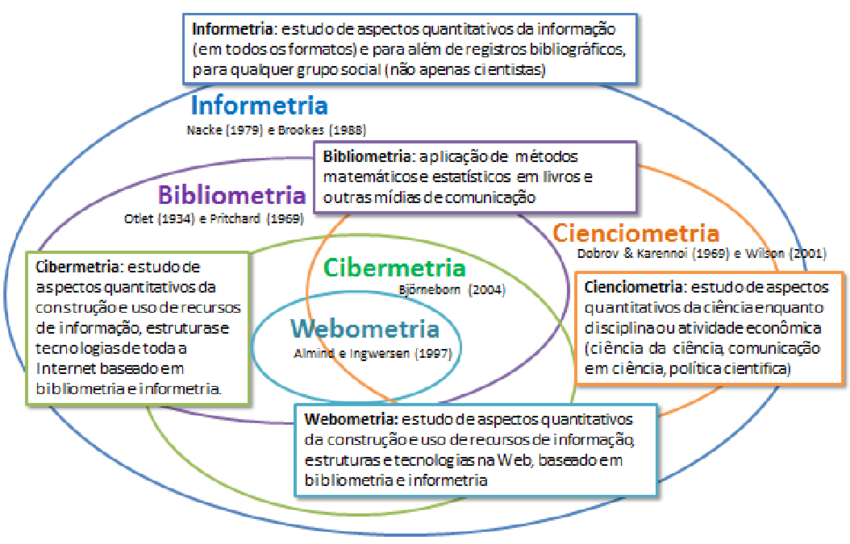
\includegraphics[trim = 0 0 0 0, clip, width=0.6\textwidth]{biblioeconomia.png}
        %\caption{.}
    \end{figure}
%*----------- notes
    \note[item]{Notes can help you to remember important information. Turn on the notes option.}
\end{frame}
%-
%*----------- SLIDE -------------------------------------------------------------
\begin{frame}[t]{Bibliometria}
    \begin{itemize}
        \item É um campo da biblioteconomia e da ciência da informação.
        \item Aplica métodos estatísticos e matemáticos para analisar e construir indicadores sobre a dinâmica e evolução da informação científica e tecnológica.
        \item Medir o impacto das publicações e dos serviços de disseminação da informação.
        \item Identificar autores e instituições mais produtivas.
        \item Todos os estudos que tentam quantificar os processos de comunicação escrita. \cite{pritchard1969statistical}
        \item Avaliar a produção científica. \cite{costa2020ciencia}
        \item Estudar relações entre a ciência e a tecnologia. \cite{maricato2010dinamica}
    \end{itemize}

    \begin{figure}
        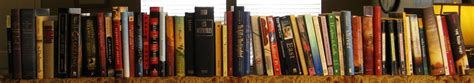
\includegraphics[trim = 0 0 0 0, clip, width=0.7\textwidth]{books-banner.jpeg}
        %\caption{.}
    \end{figure}
   
    % \begin{columns}[t]
    %     \column{.45\textwidth}
    %         detalhar sistemas em subconjuntos\\
    %         listar possíveis modos de falhas\\
    %         analisar cada modo de falha, juntamente com suas possíveis causas e sintomas
    %     \column{.45\textwidth}
    %         estimar os efeitos de cada modo de falhas\\
    %         estimar a criticidade de cada efeito\\
    %         identificar ações para minimizar falhas
    % \end{columns}
%*----------- notes
    \note[item]{Notes can help you to remember important information. Turn on the notes option.}
\end{frame}
%-
%*----------- SLIDE -------------------------------------------------------------
\begin{frame}[t]{Principais autores}
    %\framesubtitle{Lei de Bradford}
    % \begin{figure}
    %     %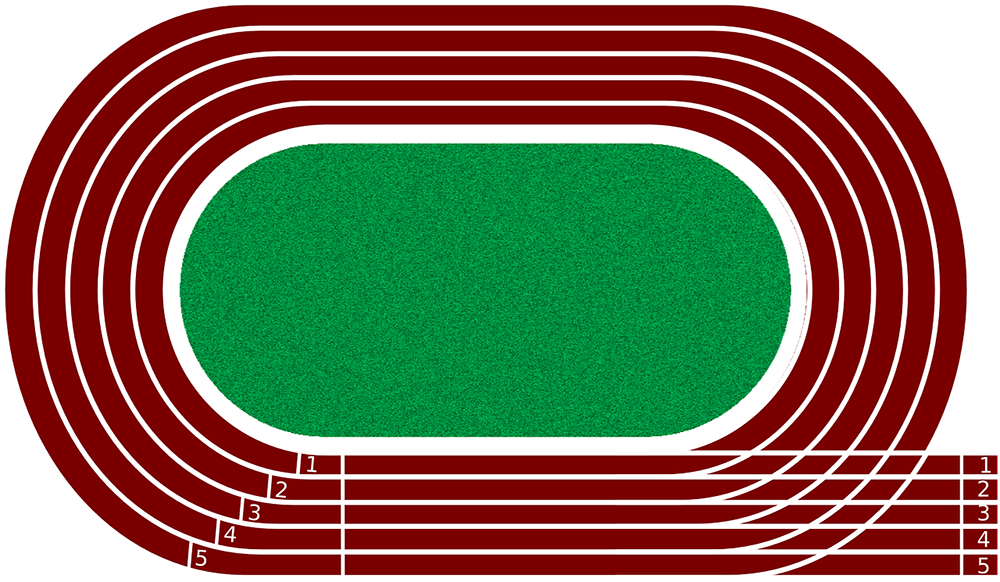
\includegraphics[width=0.7\textwidth]{pista_corrida}
       
    %     \roundpic[xshift=0cm,yshift=0cm]{3cm}{7cm}{pista_corrida}
          
    %     \caption{Formato de um pista de corrida.\cite{agostini2007}}
    % \end{figure}

    \begin{columns}
        %\column{.01\textwidth}
        \column{.33\textwidth}
            \centering
            \roundpic[xshift=0cm,yshift=-0.5cm]{5cm}{7cm}{Samuel_Clemente_Bradford}
            Samuel Clement Bradford\\
            1934
        \column{.33\textwidth}
            \centering
            \roundpic[xshift=0cm,yshift=0cm]{5cm}{7cm}{Alfredo-Lotka}
            Alfred James Lotka\\
            1926
        \column{.33\textwidth}
            \centering
            \roundpic[xshift=0cm,yshift=-1cm]{5cm}{7cm}{George-Zipf}
            George Kingsley Zipf\\
            1940
    \end{columns}

%*----------- notes
    \note[item]{Notes can help you to remember important information. Turn on the notes option.}
\end{frame}
%-
%*----------- SLIDE -------------------------------------------------------------
\begin{frame}[t]{As principais leis bibliométricas}
    \framesubtitle{Lei de Bradford - produtividade de periódicos}
    % \begin{figure}
    %     %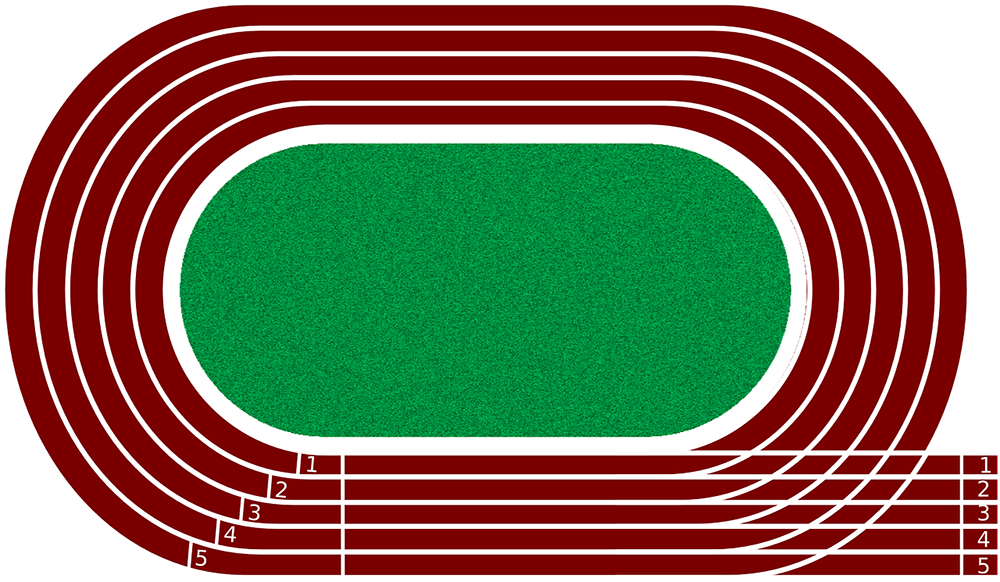
\includegraphics[width=0.7\textwidth]{pista_corrida}
       
    %     \roundpic[xshift=0cm,yshift=0cm]{3cm}{7cm}{pista_corrida}
          
    %     \caption{Formato de um pista de corrida.\cite{agostini2007}}
    % \end{figure}

    \begin{columns}
        \column{.1\textwidth}
        \column{.3\textwidth}

        \begin{figure}
            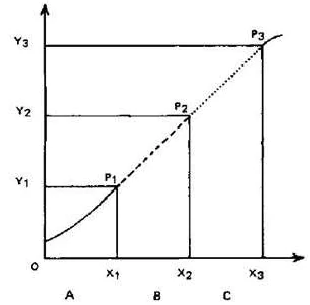
\includegraphics[trim = 0 0 0 0, clip, width=0.7\textwidth]{bradford-2.png}
            %\caption{.}
        \end{figure}

        \centering
        $F(x) = a + b \log x$
        \column{.69\textwidth}
        A lei de Bradford objetiva conhecer o núcleo de periódicos produzidos em determinado tema.\\
        \scriptsize{
            Bradford realiza uma série de estudos que culminam, em 1934, com a formulação da \textbf{lei da dispersão}.\\
            O autor percebe que, numa coleção de periódicos sobre geofísica, existe sempre um núcleo menor de periódicos relacionados de maneira estreita, sendo que o número de perióidocs em cad zona aumenta, enquanto a produtividade diminui.\\
            Analisando 326 períodicos, ele descobriu que 9 periódicos continham 429 artigos, 59 continham 499 e 258 continham 404 artigos.
        }
    \end{columns}

    \vspace*{0.2cm}
    \begin{itemize}
        \item Medir produtividade dos periódicos
        \item Estabelecer núcleo e as áreas de dispersão 
        \item Permite fazer a estimativa do grau de relevância das revistas de conhecimentos
    \end{itemize}
%*----------- notes
    \note[item]{Notes can help you to remember important information. Turn on the notes option.}
\end{frame}
%-
%*----------- SLIDE -------------------------------------------------------------
\begin{frame}[t]{As principais leis bibliométricas}
    \framesubtitle{Lei de Lotka - produtividade científica de autores}
    % \begin{figure}
    %     %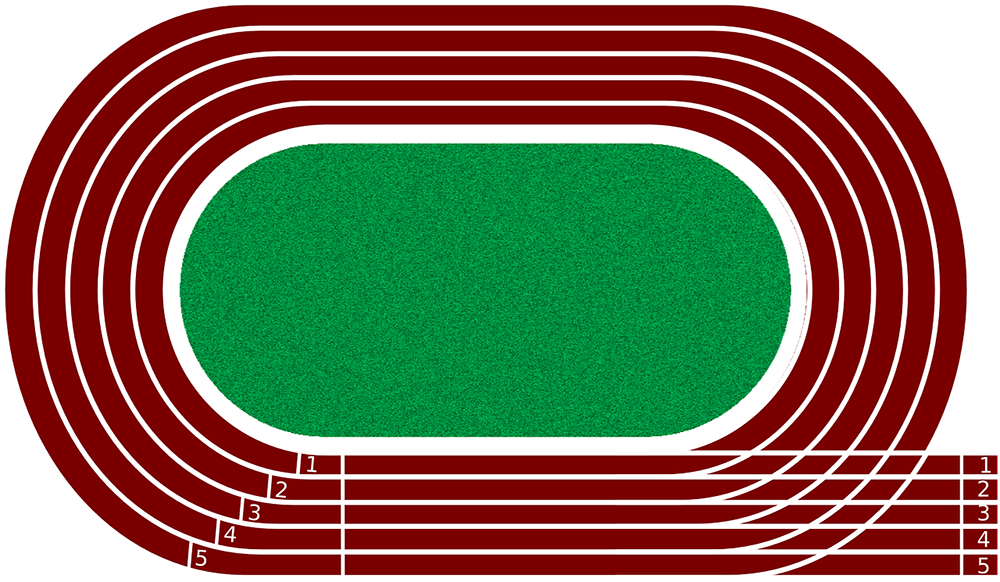
\includegraphics[width=0.7\textwidth]{pista_corrida}
       
    %     \roundpic[xshift=0cm,yshift=0cm]{3cm}{7cm}{pista_corrida}
          
    %     \caption{Formato de um pista de corrida.\cite{agostini2007}}
    % \end{figure}

    \begin{columns}
        \column{.01\textwidth}
        \column{.5\textwidth}

        \begin{figure}
            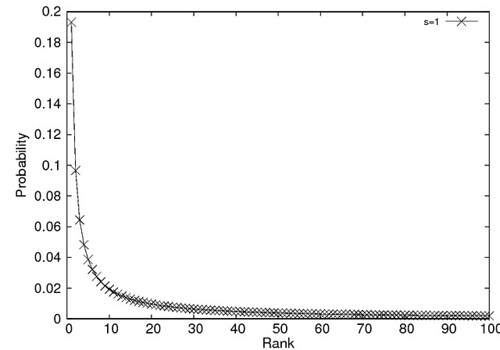
\includegraphics[trim = 0 0 0 0, clip, width=0.6\textwidth]{lotka}
            %\caption{.}
        \end{figure}

        \centering
        $Y = \frac{C}{X^n}$\\
        $Y$ \scriptsize{é a frequência relativa de autores com $X$ publicações.}\\
        $C$ \scriptsize{é a constante que depende da área $X$ é o número de publicações.}

        \column{.49\textwidth}
        A lei de Lotka visa definir as maiores contribuições de pesquisadores em determinadas áreas do conhecimento.\\
        %\scriptsize{
            Lotka descobriu que uma larga proporção da literatura científica é produzida por um pequeno número de autores, e um grande número de pequenos produtores se iguala, em produção, ao reduzido número de grandes produtores.
        %}
    \end{columns}

    \vspace*{0.2cm}

%*----------- notes
    \note[item]{Notes can help you to remember important information. Turn on the notes option.}
\end{frame}
%-
%*----------- SLIDE -------------------------------------------------------------
\begin{frame}[t]{As principais leis bibliométricas}
    \framesubtitle{Lei de Zipf - frequência de palavras}
    % \begin{figure}
    %     %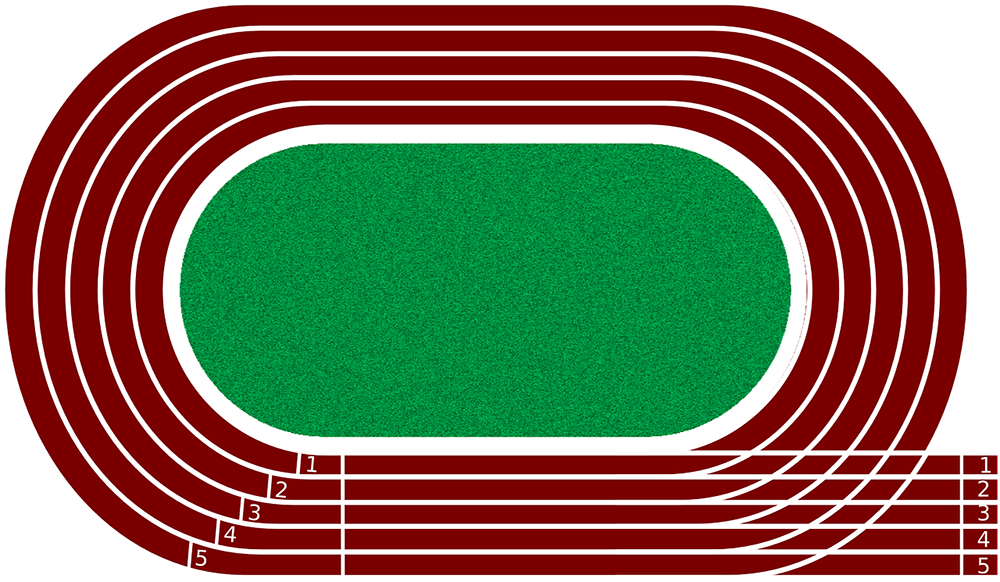
\includegraphics[width=0.7\textwidth]{pista_corrida}
       
    %     \roundpic[xshift=0cm,yshift=0cm]{3cm}{7cm}{pista_corrida}
          
    %     \caption{Formato de um pista de corrida.\cite{agostini2007}}
    % \end{figure}

    \begin{columns}
        \column{.01\textwidth}
        \column{.5\textwidth}

        \begin{figure}
            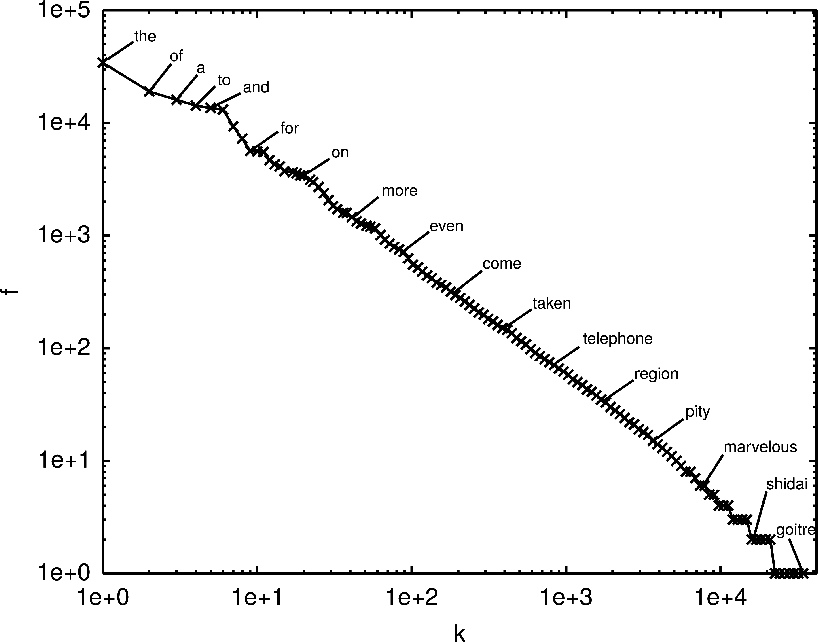
\includegraphics[trim = 0 0 0 0, clip, width=0.5\textwidth]{Figura-1-Lei-de-Zipf-no-Ingles-escrito-dados-do-OANC-Rank-k-versus-frequencia-de.png}
            %\caption{.}
        \end{figure}

        \centering
        $f(n) = \frac{K}{n}$\\
        $f(n)$ \scriptsize{é a frequência de ocorrência de uma palavra}\\
        $n$ \scriptsize{é a ordem de frequência}
        $K$ \scriptsize{é a constante}\\

        \column{.49\textwidth}
        A lei de Zipf pontua a frequência com que certas palavras aparecem nos textos científicos de maneira a definir sua representatividade neste contexto.\\
        \scriptsize{
            Diante desta visão, Zipf formulou o \textbf{princípio do menor esforço}: existe uma economia do uso de palavras, e se a tendência é usar o mínimo significa que elas não vão se dispersar, pelo contrário, uma mesma palavra vais ser usada muitas vezes; as palavras mais usadas indicam o assunto do documento.
        }
    \end{columns}

    \vspace*{0.2cm}
    \begin{itemize}
        \item Trata e mede a frequência de ocorrência de palavras em vários textos.
        \item As palavras mais usadas indicam o assunto.
    \end{itemize}
%*----------- notes
    \note[item]{Notes can help you to remember important information. Turn on the notes option.}
\end{frame}
%-
%*----------- SLIDE -------------------------------------------------------------
\begin{frame}[t]{O fator de impacto}
    %\transboxin[duration=1,direction=30]
    \large{Medida que reflete o número médio de citações de artigos científicos publicados.}\\

    \vspace*{0.2cm}
	Tem como objetivo avaliar a importância de um dado periódico em sua área.

    \begin{figure}
        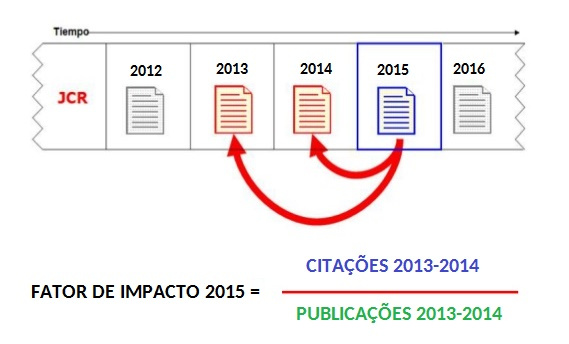
\includegraphics[trim = 0 0 0 0, clip, width=0.6\textwidth]{fi.jpg}
        %\caption{.}
    \end{figure}
%*----------- notes
    \note[item]{Notes can help you to remember important information. Turn on the notes option.}
\end{frame}
%-
%*----------- SLIDE -------------------------------------------------------------
\begin{frame}{Principais estudos da Bibliometria}
    % \begin{table}[ht!]
    %     \centering
    %         \caption{PERCENTUAL DE CONCLUSÃO POR EQUIPE}
    %         \begin{tabular}{|l|c|c|c|c|} \hline
    %             \textbf{EQUIPE}&\textbf{04/05}&\textbf{11/05}&\textbf{18/05}&\textbf{25/05}\\ \hline
    %             RAJA & 17\% &32\% & &  \\ \hline
    %             BORG & 0\% &41\% & &  \\ \hline
    %             TIMON-HM & 5\% &47\% & &  \\ \hline
    %         \end{tabular}
    % \end{table}

	\begin{table}[ht!]
		%\scalefont{0.7}
        \resizebox{0.9\textwidth}{!}{
		\begin{tabular}{|l|c|l|}
            \hline
            \multicolumn{1}{|c|}{\textbf{Leis e Princípios}} & \textbf{Foco de Estudo} & \multicolumn{1}{c|}{\textbf{Principais Aplicações}}                                                                         \\ \hline
            Lei de Bradford                                  & periódicos               & \begin{tabular}[c]{@{}l@{}}estimar o grau de relevância de periódicos\end{tabular}         \\ \hline
            Lei de Lotka                                     & autores                  & \begin{tabular}[c]{@{}l@{}}estimar o grau de relevância de autores\end{tabular}            \\ \hline
            Leis de Zipf                                     & palavras                 & \begin{tabular}[c]{@{}l@{}}indexação automática de artigos científicos\\ e tecnológicos\end{tabular}                        \\ \hline
            Fator de Impacto               & citações                 & \begin{tabular}[c]{@{}l@{}}estimar o grau de relevância de artigos, \\ cientistas e periódicos científicos\end{tabular} \\ \hline
            Acoplamento Bibliográfico                        & citações                 & \begin{tabular}[c]{@{}l@{}}estimar o grau de ligação de dois ou mais \\ artigos\end{tabular}                                \\ \hline
            Co-citação                                       & citações                 & \begin{tabular}[c]{@{}l@{}}estimar o grau de ligação de dois ou mais \\ artigos\end{tabular}                                \\ \hline
            Obsolescência da Literatura                      & citações                 & \begin{tabular}[c]{@{}l@{}}estimar o declínio da literatura de \\ determinada área do conhecimento\end{tabular}             \\ \hline
            Vida-média                                       & citações                 & \begin{tabular}[c]{@{}l@{}}estimar a vida-média de uma unidade da\\  literatura de dada área do conhecimento\end{tabular}   \\ \hline
		\end{tabular}
        }
	\end{table}

%*----------- notes
\note[item]{Notes can help you to remember important information. Turn on the notes option.}
\end{frame}
%-
%*----------- SLIDE -------------------------------------------------------------
\begin{frame}[c]{}

    \centering
    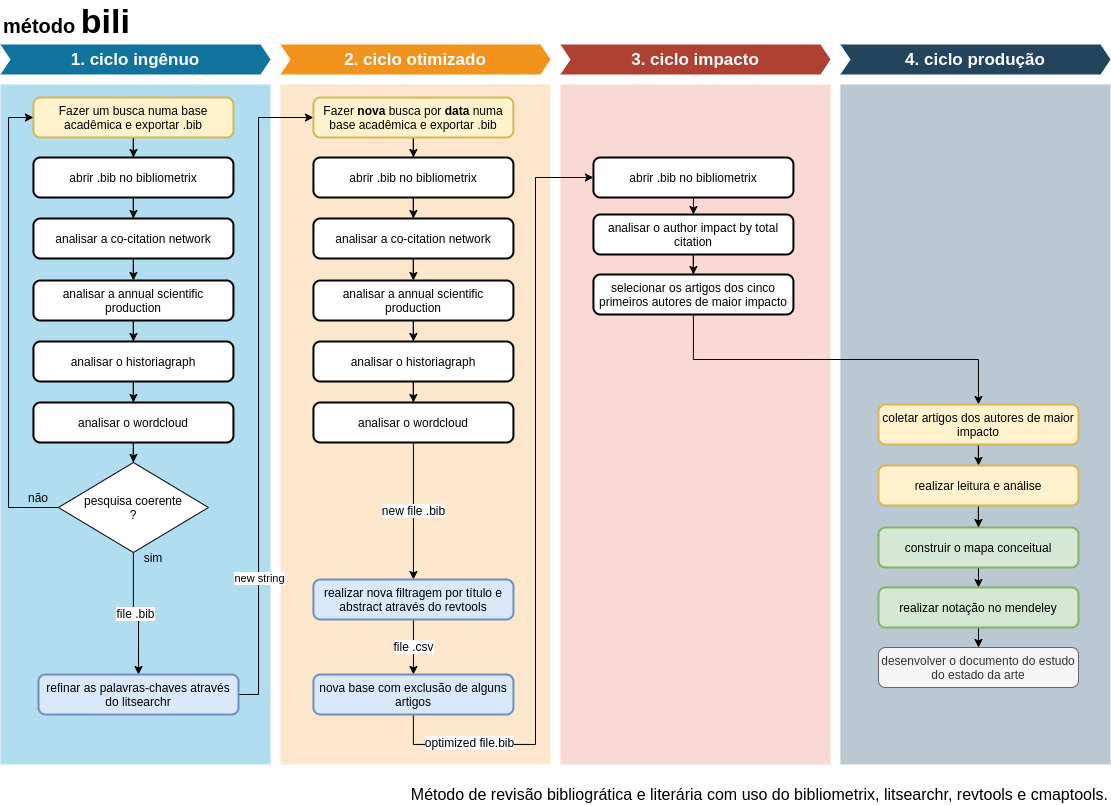
\includegraphics[width=.85\textwidth, trim= 0 30 0 0, clip]{revisão bibliogrática Diagram.png}
    
        
    % \begin{tikzpicture}[remember picture,overlay]
    %     \draw[red,very thick] (cmark) circle[x radius=8mm,y radius=4mm]; 
    % \end{tikzpicture}
%*----------- notes
    \note[item]{Notes can help you to remember important information. Turn on the notes option.}
\end{frame}
%-